\section{Commande logique}
\subsection{Principe de base}
\label{sec-cmd_principes_base}
Le moteur de défis solaire est un moteur brushless triphasé (BLDC) piloté par un "asservissement à la position suivante".
Il s'agit, à l'aide d'un codeur, d'obtenir la position absolue du moteur et d'en déduire la commande de phases correspondante à la position en cours.
Il suffit ensuite de décaller cette commande dans une direction ou l'autre pour faire tourner le moteur qui suivra la commande.

Ce mécanisme est à l'origine de la commande des moteurs synchrones, mais la conaissance de la position du moteur permet d'éviter le phénomène de décrochage.

\paragraph{}
Par construction, on a 3 bobines pour 4 pôles (aimants). Ainsi, lors d'une rotation, on a les déplacements présentés 
\cref{fig-bobines_vs_aimants} entre les bobines et les aimants.

Sur cette figure, la première ligne représente la position des aimants. $P$ signifie que le pôle positif est présenté au stator tandis que $N$ indique que le pôle négatif est présenté au stator.
Les zones en hachuré indiquent qu'il s'agit d'une position dans laquelle une bobine ne devrait pas être alimentée.

Les dégradés de couleurs indiquent qu'une bobine à cette position devrait être polarisée dans le sens positif (rouge) ou négatif (bleu) afin de déplacer les bobines vers la droite.
Le fait que les zones de couleurs soient dégradées représente le fait qu'il est plus efficace d'alimenter les bobines lorsqu'elles sont proches des aimants (couleur intense) plutôt qu'entre deux aimants (blanc).
Enfin, chaque ligne représente l'écoulement du temps, en direction du bas.
Les lettres présentes dans la partie basse de la \cref{fig-bobines_vs_aimants} correspondent à la position de la phase correspondant à la lettre.
\begin{figure}[h]
    \centering
    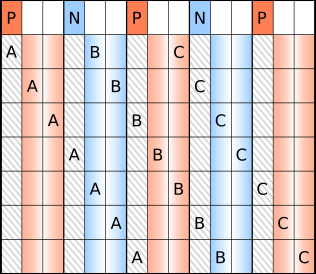
\includegraphics{png/phases_aimants_switching.png}
    \caption{Vision du déplacement vers la droite des bobines vis-à-vis des aimants}
    \label{fig-bobines_vs_aimants}
\end{figure}

Les six étapes que l'on peut voir \cref{fig-bobines_vs_aimants} correspondent à des commandes de phases.
Afin de correspondre à l'implémentation électronique du bloc de commande, on considèrera pour les trois phases \pha, \phb et \phc des signaux $\mathit{Phase}_-$ et $\mathit{Phase}_+$
qui correspondent respectivement à la mise à la masse et à la mise sous tension de la phase.

\paragraph{}
La \cref{fig-bobines_vs_aimants} correspond donc à la succession des signaux de commande présentée \cref{fig-wave_phase_drive}. 
On remarquera notamment que les signaux \phstate{x}{\phhi} et \phstate{x}{\phlo} d'une même phase ne sont \emph{jamais} pilotés en même temps.
En effet, d'un point de vue électronique, cela reviendrait à réaliser un court-circuit. 

\begin{figure}[h]
    \centering
    \import{pdftex/}{wave_phase_drive.pdf_tex}
    \caption{Signaux de pilotage des phases}
    \label{fig-wave_phase_drive}
\end{figure}

Chaque partie du chronogramme de la \cref{fig-wave_phase_drive} correspond à une configuration $P^1_+ + P^2_-$ différente.
On appellera par la suite ces configurations des \emph{pas de commande}.
Lors d'un fonctionnement normal, il n'est pas possible de sauter des pas, à moins que le moteur n'aille trop vite pour le système de commande.  

\subsection{Détermination de la longueur des pas de phase}
Le codeur utilisé pour l'asservissement du moteur est un codeur incrémental utilisant des signaux ABI\todo{wave si pas flemme}.
Afin d'établir un système de commande, il faut déterminer \dnabi le nombre d'évènement ABI entre chaque changement de configuration de phase.

\paragraph{}
On considère un moteur avec 3 bobines pour 4 aimants tel que précédemment defini ainsi que la \cref{fig-bobines_vs_aimants}.
Si l'on a au total \naimants aimants pour \nbobines bobines, il faudra réaliser \nseq fois la séquence présentée \cref{fig-wave_phase_drive} où
$$\nseq = \frac{\naimants}{2}$$

Soit un nombre $\nstep$ de pas de pilotage de phases par tour de roue défini par:
$$\nstep = 6 \times \nseq$$

Enfin, si l'on considère \nabi le nombre d'évènement produit par le codeur incrémental par tour de roue, on a :
$$\dnabi = \cfrac{\nabi}{\nstep} = \cfrac{\nabi}{\cfrac{6\times\naimants}{2}} = \cfrac{\nabi}{3\times\naimants}$$

Considérant le codeur incrémental AS5047P configuré pour générer 300 impulsions par tour soit 1200 évenements exploitables par tour de roue.
Soit donc 
$$\dnabi = \frac{1200}{3\times40} = 10$$

Il est donc nécessaire de changer de configuration de phases tous les 10 évènements ABI.

\paragraph{}
Notons que si la géométrie du moteur change et que l'on souhaite modifier le nombre d'aimants/de bobines, \dnabi est inversement proportionnel au nombre d'aimants \naimants.
Dans cette configuration, on pourra donc réduire le nombre d'aimants de n'importe quelle valeur tout en conservant un nombre entier d'étapes ABI par pas de commande.

\subsection{Principe de la commande PWM directe}

Afin d'avoir un système fonctionnel en toute circonstance, notamment lorsque le moteur n'est pas en rotation, 
une solution simple consiste à gérer la puissance via une modulation de largeur d'impulsion (MLI ou PWM) indépendamment de la position du moteur.
On a alors deux commandes différentes et dissociées :
\begin{itemize}
    \item Une commande de sélection de phase, dépendant de la position du moteur,
    \item Une commande de puissance, uniquement dépendante de l'utilisateur.
\end{itemize}

Cette commande consiste à effectuer un ET logique entre la sélection de phase et la commande de puissance.

\paragraph{}
Cette méthode présente un certain nombre d'inconvenients, notamment une possibilité de stresser l'électronique de puissance ("glitchs" de commande) et une commande sous-optimale (voir \cref{sec-cmd_limite_position}).
Cependant, cette méthode est extrèmement fiable et permet un démarrage à l'arrêt. 

\paragraph{}
Cette méthode sera donc utilisée pour lancer le moteur ou lorsque le moteur tourne trop lentement pour pouvoir être piloté autrement.

\subsection{Principe de la commande aux limites de position}
\label{sec-cmd_limite_position}
Afin d'être au maximum d'efficacité lors des commandes, on tentera de piloter les phases comme indiqué dans la \cref{sec-cmd_principes_base}.

\paragraph{}
Le détail de cette commande est montré \cref{fig-wave_drive_wrt_abi}. 
En considérant un sens de rotation normal, un signal de configuration de phase quelconque devra rester actif pendant deux pas de commande consécutifs.
Afin d'éviter tout "collage" à l'aproche de l'aimant (fin de chronogramme), on pourra prendre un évènement ABI de marge pour désactiver la commande prématurément (représenté en orange).
Afin de réguler la puissance fournée, on réalisera une modulation de largeur d'impulsion (PWM) mais dont la periode inactive sera centrée sur le moment éloigné des aimants, entre les deux pas de commande.
On utilisera pour cela une valeur de "niveau de puissance" associant le pas ABI à un seuil, en fonction du pas de commande en cours.
Pour piloter la puissance, il suffira alors d'activer la puissance tant que la commande est inferieure au niveau de puissance.

Afin de permettre une extinction totale de la puissance, on utilisera une comparaison stricte (commande strictement infèrieure au seuil).

\begin{figure}[h]
    \centering
    \def\svgwidth{17cm}
    \small
    \import{pdftex/}{wave_drive_puissance.pdf_tex}
    \caption{Exemple de pilotage de la puissance vis-à-vis d'un encodeur ABI}
    \label{fig-wave_drive_wrt_abi}
\end{figure}


\subsection{Configuration initiale et prise d'origine}
Afin de régler la position initiale du codeur, on essaiera de se placer dans une position mécaniquement stable.
Une telle position ne peut être atteinte en utilisant une configuration normale de pilotage du moteur de la forme $(\phstate{x}{\phhi},\phstate{y}{\phlo},\phstate{z}{\phoff})$ qui est magnétiquement stable mais mécaniquement instable.

On choisira plutôt une configuration de la forme $(\phstate{x}{\phhi},\phstate{y}{\phlo},\phstate{z}{\phlo})$, permettant de positionner la phase \phase{x} en face d'un pôle P

Cette position doit ensuite être associée à une valeur "zéro" du codeur et l'initialisation du système peut se faire.
Cette position correspond à un pas ABI \initabipos valant :
$$\initabipos = \frac{\dnabi}{2}$$
